\apendice{Especificación de diseño}
\label{sec:appendixC}

\section{Introducción}

En este apéndice se describen los diseños de nodos que permiten cumplir con los objetivos
 generales del proyecto y los requisitos funcionales definidos previamente. 

\section{Diseño de la extensión KNIME Moodle Integration}

Se ha diseñado la extensión KNIME Moodle Integration con los siguientes nodos individuales: 

\begin{itemize}
  \item \node{Moodle Connector}. Cubre los requisitos especificados en RF-1 (RF-1.1 y RF-1.2). 
  \item \node{Moodle Courses}. Cubre los requisitos especificados en RF-2 (RF-2.1 y RF-2.2).
  \item \node{Moodle Users}. Cubre los requisitos especificados en RF-3 (RF-3.1, RF-3.2, RF-3.3 y RF-3.4).
  \item \node{Moodle Reports Logs}. Cubre los requisitos especificados en RF-4. 
  \item \node{Moodle Reports Grades}. Cubre los requisitos especificados en RF-5. 
  \item \node{Moodle Reports Quizzes}. Cubre los requisitos especificados en RF-6. 
\end{itemize}

En el diseño se han tenido en cuenta también los requisitos no funcionales RNF-1, RNF-2 y RNF-3. 
\

\begin{figure}[!h]
	\centering
	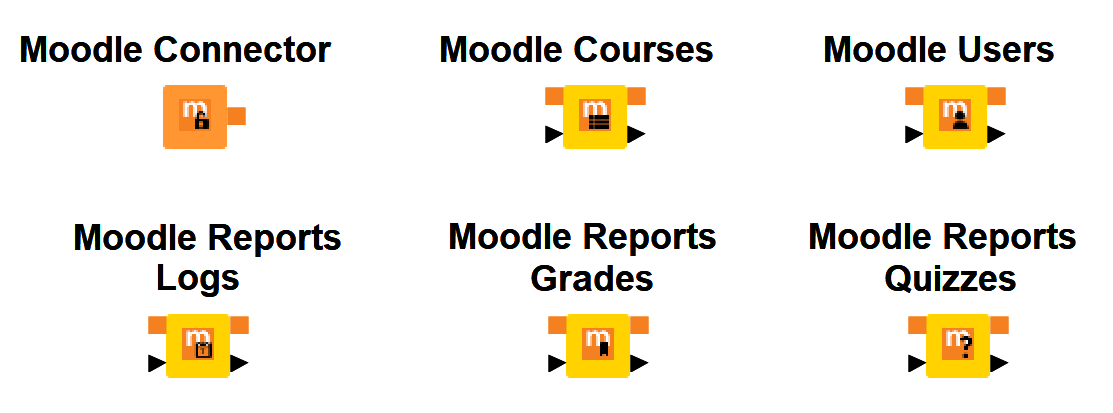
\includegraphics[width=1\textwidth]{img/nodes_moodle_todos.png}
	\caption{Nodos implementados en la extensión \node{KNIME Moodle Integration}.}
	\label{fig:moodlenodesall}
\end{figure}
\FloatBarrier


Se describe a continuación el diseño de cada nodo implementado. 

\newpage
\subsection{Diseño del nodo Moodle Connector}

El nodo \node{Moodle Connector} establece la conexión con una plataforma Moodle. Requiere una cuenta con perfil de profesor (RF-1.1). 
Requiere que la plataforma Moodle tenga activado el acceso a la aplicación móvil (RF-1.1). 
\

El nodo devuelve a través de un puerto de salida la información de sesión, de forma que, conectada a otros nodos de la extensión, 
estos pueden extraer información de Moodle sin necesidad de volver a conectarse.
\ 

El nodo tiene la siguiente \textbf{estructura}:

\begin{itemize}
	\item \textbf{Puertos de entrada}: 
    \begin{itemize}
		\item Sin puertos de entrada. 
   	\end{itemize}

	\item \textbf{Puertos de salida}: 
    \begin{itemize}
		\item \textbf{0. Moodle Courses}. Una conexión que se puede utilizar para acceder a la API de Moodle. 
   	\end{itemize}

\end{itemize}

\begin{figure}[!h]
	\centering
	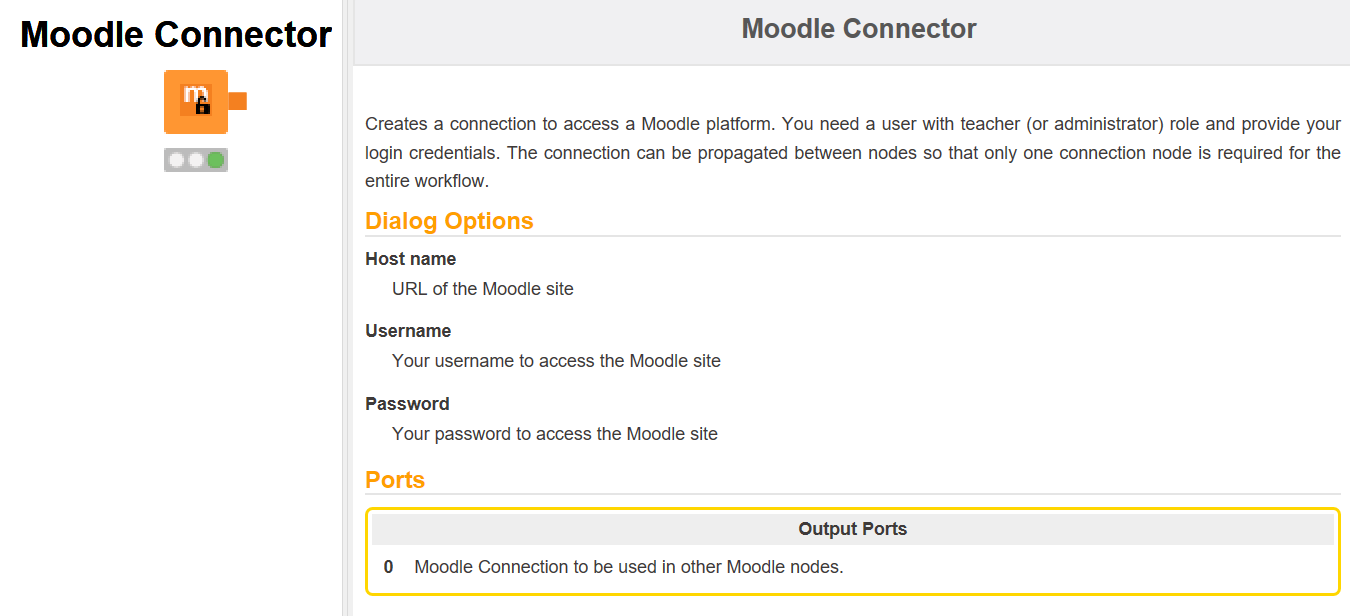
\includegraphics[width=1\textwidth]{img/nodes_moodle_connector.png}
	\caption{Nodo \node{Moodle Connector}. Descripción.}
	\label{fig:moodleconnector}
\end{figure}
\FloatBarrier


El nodo permite la siguiente \textbf{configuración}: 

\begin{itemize}
   \item \textbf{Host name}. URL de la plataforma Moodle, empezando por http o https. 
   \item \textbf{Username}. Nombre de usuario de acceso a Moodle.
   \item \textbf{Password}. Contraseña de acceso a Moodle.
\end{itemize}

\begin{figure}[!h]
	\centering
	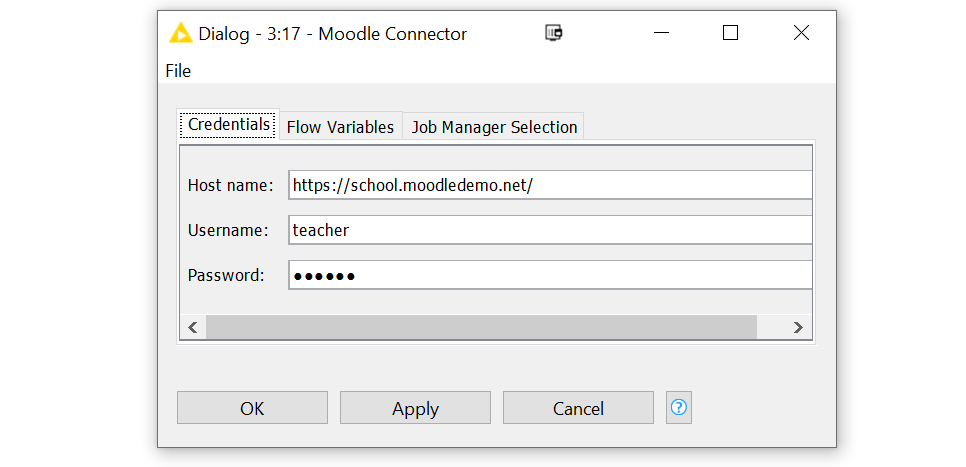
\includegraphics[width=1\textwidth]{img/nodes_moodle_connector_settings.png}
	\caption{Nodo \node{Moodle Connector}. Configuración.}
	\label{fig:moodleconnector_settings}
\end{figure}
\FloatBarrier

\hphantom{ }

\newpage    
\subsection{Diseño del nodo Moodle Courses}

El nodo \node{Moodle Courses} extrae información de cursos. Permite obtener uno o varios cursos según su id (RF-2.1) o todos 
los cursos dentro de las categorías especificadas (RF-2.2). 
\

El nodo tiene la siguiente \textbf{estructura}:

\begin{itemize}
	\item \textbf{Puertos de entrada}: 
    \begin{itemize}
		\item \textbf{0. Moodle Connection}. Conexión obtenida desde el nodo \node{Moodle Connector}. 
		\item \textbf{1. Input table}. Tabla de entrada con información de filtrado. 
		Columna con identificador de cursos y columna con identificador de categorías. Aunque el filtrado no es obligatorio, sí se 
		requiere añadir un nodo que defina la tabla de entrada. 
   	\end{itemize}

	\item \textbf{Puertos de salida}: 
    \begin{itemize}
		\item \textbf{0. Moodle Connection}. Devuelve la conexión para facilitar su transferencia al siguiente nodo del flujo de trabajo. 
		\item \textbf{1. Output table}. Tabla de salida con la información de los cursos. 
   	\end{itemize}

\end{itemize}

\begin{figure}[!h]
	\centering
	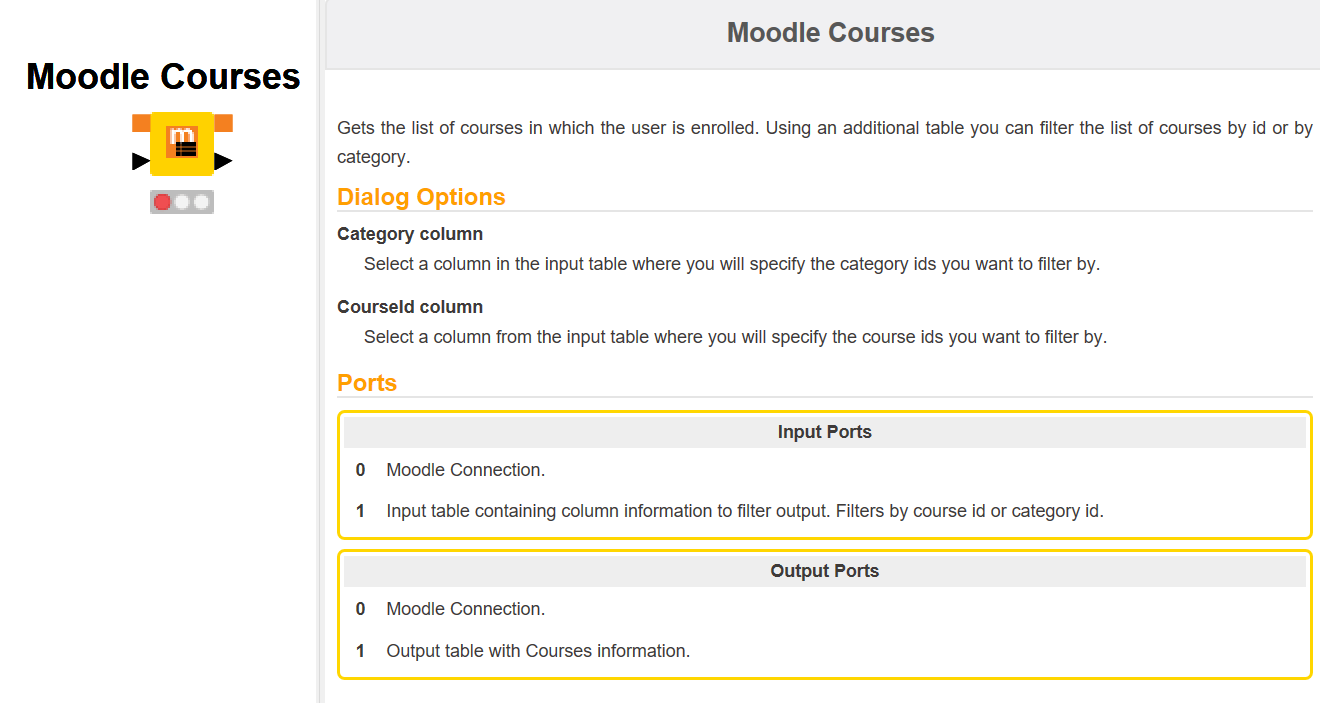
\includegraphics[width=1\textwidth]{img/nodes_moodle_courses.png}
	\caption{Nodo \node{Moodle Courses}. Descripción.}
	\label{fig:moodlecourses}
\end{figure}
\FloatBarrier



El nodo permite la siguiente \textbf{configuración}: 

\begin{itemize}
   \item \textbf{Category column}. Permite seleccionar la columna en la que se encuentran las categorías por las que se desea filtrar. Es opcional. 
   \item \textbf{CourseId column}. Permite seleccionar la columna en la que se encuentran los identificadores de cursos por los que se desea filtrar. Es opcional. 
\end{itemize}

\begin{figure}[!h]
	\centering
	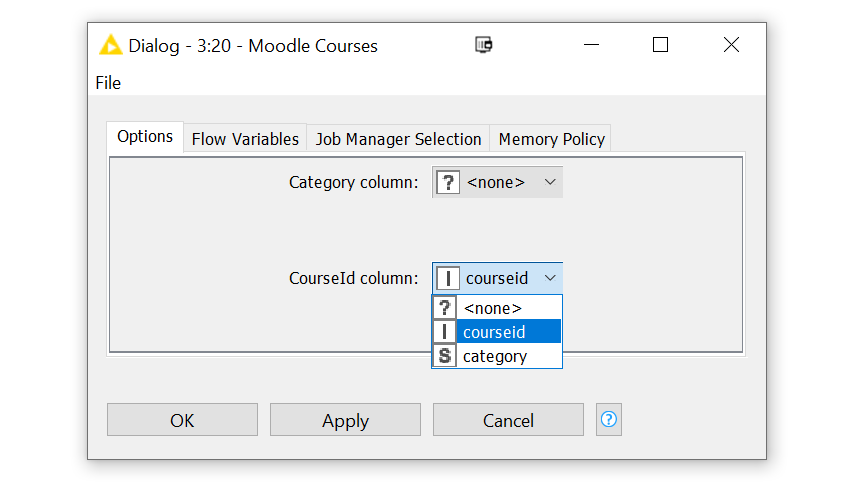
\includegraphics[width=1\textwidth]{img/nodes_moodle_courses_settings.png}
	\caption{Nodo \node{Moodle Courses}. Configuración.}
	\label{fig:moodlecourses_settings}
\end{figure}
\FloatBarrier

En la tabla~\ref{tab:moodle_courses_desc} se muestra la estructura de los datos devueltos por cada curso encontrado en la plataforma Moodle: 

\begin{table}[!h]
	\begin{center}
		\begin{tabular}{p{0.3\textwidth}p{0.1\textwidth}p{0.6\textwidth}}
			\toprule
			\textbf{Columna} & \textbf{Tipo} & \textbf{Descripción}\\
			\otoprule
			\textbf{courseid} & integer & ID del curso \\
         \hline
			\textbf{shortname} & string & Descripción corta del curso \\
         \hline
         \textbf{fullname} & string & Nombre completo del curso \\
         \hline
         \textbf{displayname} & string & Nombre del curso que se muestra en el aula \\
         \hline
         \textbf{enrolledusercount} & string & Número de alumnos registrados en el curso \\
         \hline
         \textbf{idnumber} & string & ID interno del curso \\
         \hline
         \textbf{visible} & boolean & Indica si el curso es visible para los estudiantes (1) \\
         \hline
         \textbf{summary} & string & Resumen o descripción del curso\\
         \hline
         \textbf{summaryformat} & boolean & Indica si el resumen tiene formato de texto asociado (1) \\
         \hline
         \textbf{format} & string & Tipo de formato del resumen \\
         \hline
         \textbf{category} & string & ID de categoría \\
         \hline
         \textbf{categoryname} & string & Nombre de la categoría \\
			\bottomrule
		\end{tabular}
	\end{center}
	\caption{Tabla de salida del nodo \node{Moodle Courses}.}
	\label{tab:moodle_courses_desc}
\end{table}
\FloatBarrier


\begin{figure}[!h]
	\centering
	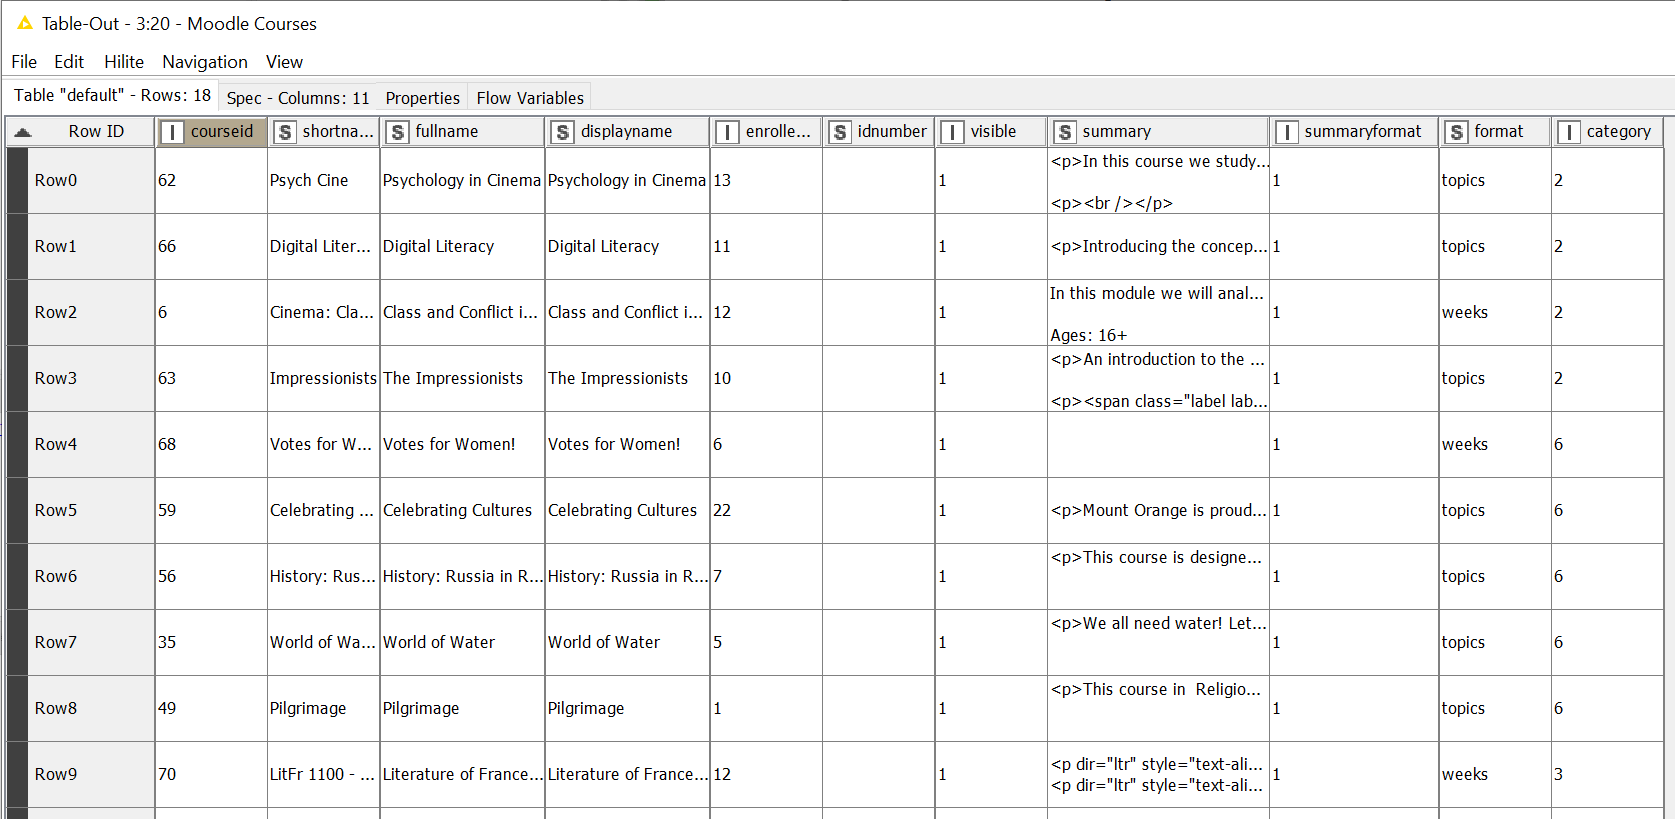
\includegraphics[width=1\textwidth]{img/nodes_moodle_courses_output.png}
	\caption{\node{Nodo Moodle Courses}. Ejemplo de salida.}
	\label{fig:moodlecourses_output}
\end{figure}
\FloatBarrier
\hphantom{ }


\newpage
\subsection{Diseño del nodo Moodle Users}

El nodo \node{Moodle Users} extrae información de usuarios según los cursos especificados (RF-3.1). 
También es posible devolver solo los usuarios con rol estudiante (RF-3.2), estimar el género de cada
usuario a partir de su nombre (RF-3.3) y anonimizar los datos personales (RF-3.4). 
\

El nodo tiene la siguiente \textbf{estructura}:

\begin{itemize}
	\item \textbf{Puertos de entrada}: 
    \begin{itemize}
		\item \textbf{0. Moodle Connection}. Conexión obtenida desde el nodo \node{Moodle Connector}. 
		\item \textbf{1. Input table}. Tabla de entrada con un listado de identificadores de cursos. 
   	\end{itemize}

	\item \textbf{Puertos de salida}: 
    \begin{itemize}
		\item \textbf{0. Moodle Connection}. Devuelve la conexión para facilitar su transferencia al siguiente nodo del flujo de trabajo. 
		\item \textbf{1. Output table}. Tabla de salida con la información de los usuarios. 
   	\end{itemize}

\end{itemize}


\begin{figure}[!h]
	\centering
	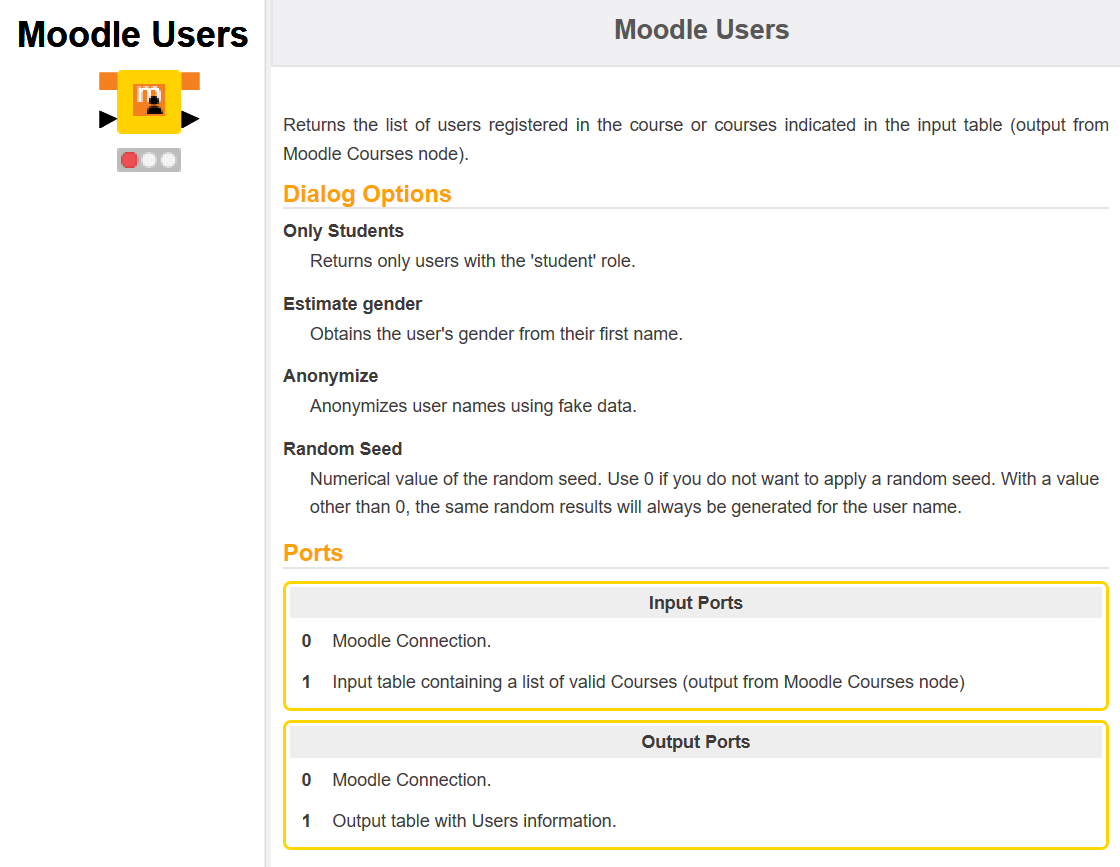
\includegraphics[width=1\textwidth]{img/nodes_moodle_users.png}
	\caption{Nodo \node{Moodle Users}. Descripción.}
	\label{fig:moodleusers}
\end{figure}
\FloatBarrier



El nodo permite la siguiente \textbf{configuración}: 

\begin{itemize}
   \item \textbf{Only students}. Si se activa, devuelve únicamente los usuarios con rol estudiante. 
   \item \textbf{Estimate gender}. Si se activa, devuelve una estimación del género del usuario (\english{male} o \english{female}). 
   \item \textbf{Anonymize}. Si se activa, devuelve el nombre y apellidos del usuario anonimizados.  
   \item \textbf{Random Seed}. Establece una semilla aleatoria para obtener un valor de nombre/apellidos anonimizado. 
   Si se deja el valor 0, los nombres/apellidos de cada usuario cambiarán con cada ejecución del nodo. 
\end{itemize}

\begin{figure}[!h]
	\centering
	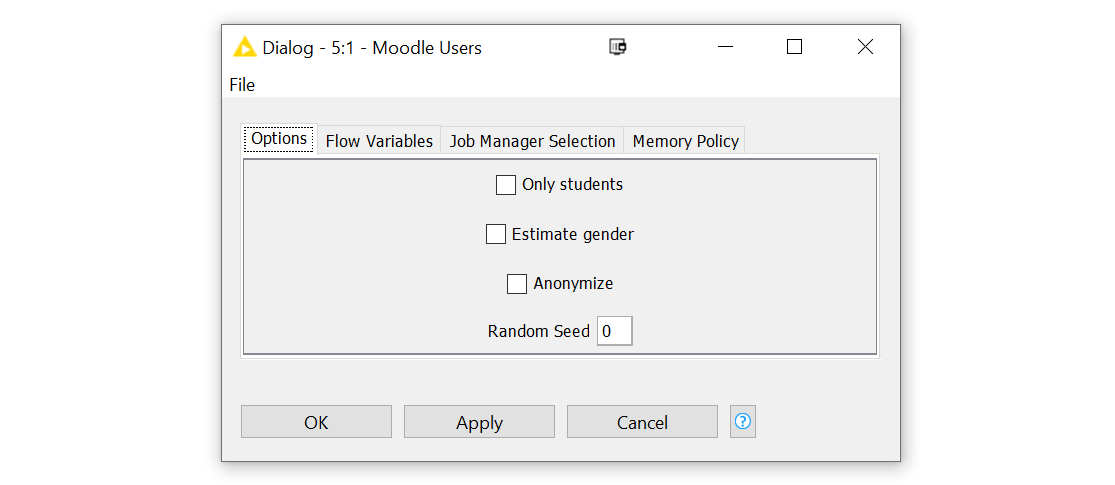
\includegraphics[width=1\textwidth]{img/nodes_moodle_users_settings.png}
	\caption{Nodo \node{Moodle Users}. Configuración.}
	\label{fig:moodleusers_settings}
\end{figure}
\FloatBarrier


En la tabla~\ref{tab:moodle_users_desc} se muestra la estructura de los datos devueltos por cada usuario: 

\begin{table}[!h]
	\begin{center}
		\begin{tabular}{p{0.25\textwidth}p{0.15\textwidth}p{0.6\textwidth}}
			\toprule
			\textbf{Columna} & \textbf{Tipo} & \textbf{Descripción}\\
			\otoprule
			\textbf{courseid} & integer & ID del curso en que el usuario está registrado\\
         \hline
			\textbf{userid} & integer & ID del usuario \\
         \hline
         \textbf{fullname} & string & Nombre completo del usuario. Puede ser el nombre real o el nombre Anonimizado, si se especifica en la configuración del nodo. \\
         \hline
         \textbf{firstaccess} & timestamp & Fecha de primer acceso al curso \\
         \hline
         \textbf{lastcourseaccess} & timestamp &  Fecha de último acceso al curso\\
         \hline
         \textbf{lastaccess} & timestamp & Fecha de último acceso a la plataforma \\
         \hline
         \textbf{roles} & string & Listado de roles del usuario, separados por coma \\
         \hline
         \textbf{country} & string & Código del país del usuario \\
         \hline
         \textbf{city} & string & Ciudad del usuario \\
         \hline
         \textbf{gender} & string & Género estimado (\english{male}, \english{female}). Esta columna es opcional, en función de la configuración del nodo. \\
			\bottomrule
		\end{tabular}
	\end{center}
	\caption{Tabla de salida del nodo \node{Moodle Users}.}
	\label{tab:moodle_users_desc}
\end{table}
\FloatBarrier

\begin{figure}[!h]
	\centering
	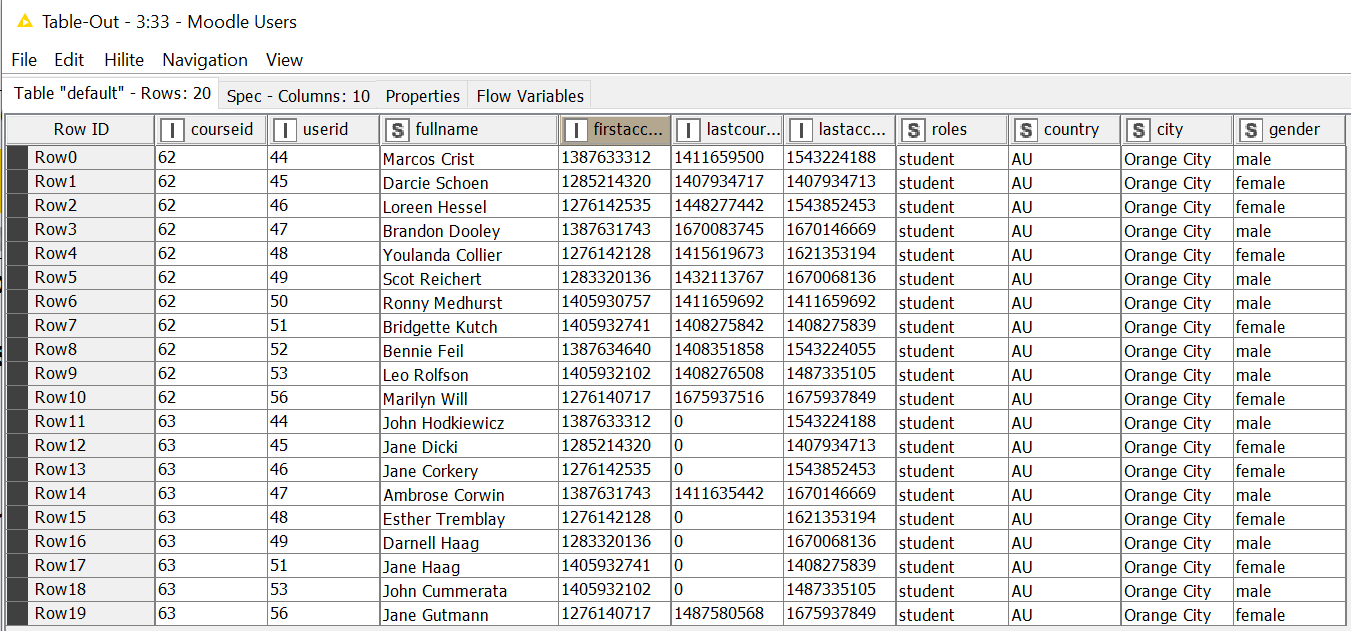
\includegraphics[width=1\textwidth]{img/nodes_moodle_users_output.png}
	\caption{Nodo \node{Moodle Users}. Salida de ejemplo. }
	\label{fig:moodleusers_output}
\end{figure}
\FloatBarrier
\hphantom{ }

\newpage
\subsection{Diseño del nodo Moodle Reports Logs}

El nodo \node{Moodle Reports Logs} extrae información de \english{logs} de la plataforma Moodle (RF-4). 
Este nodo está diseñado para poder extraer logs de forma homogénea aunque provengan de diferentes
fuentes dentro de Moodle (\english{Logs, Live logs, Activity Reports, Overview Statistics, Course Participation, Activity completion, Statistics, etc.})

\

El nodo tiene la siguiente \textbf{estructura}:

\begin{itemize}
	\item \textbf{Puertos de entrada}: 
    \begin{itemize}
		\item \textbf{0. Moodle Connection}. Conexión obtenida desde el nodo \node{Moodle Connector}. 
		\item \textbf{1. Input table}. Tabla de entrada con un listado de identificadores de cursos. 
   	\end{itemize}

	\item \textbf{Puertos de salida}: 
    \begin{itemize}
		\item \textbf{0. Moodle Connection}. Devuelve la conexión para facilitar su transferencia al siguiente nodo del flujo de trabajo. 
		\item \textbf{1. Output table}. Tabla de salida con la información de los \english{logs} o eventos. 
   	\end{itemize}

\end{itemize}

\begin{figure}[!h]
	\centering
	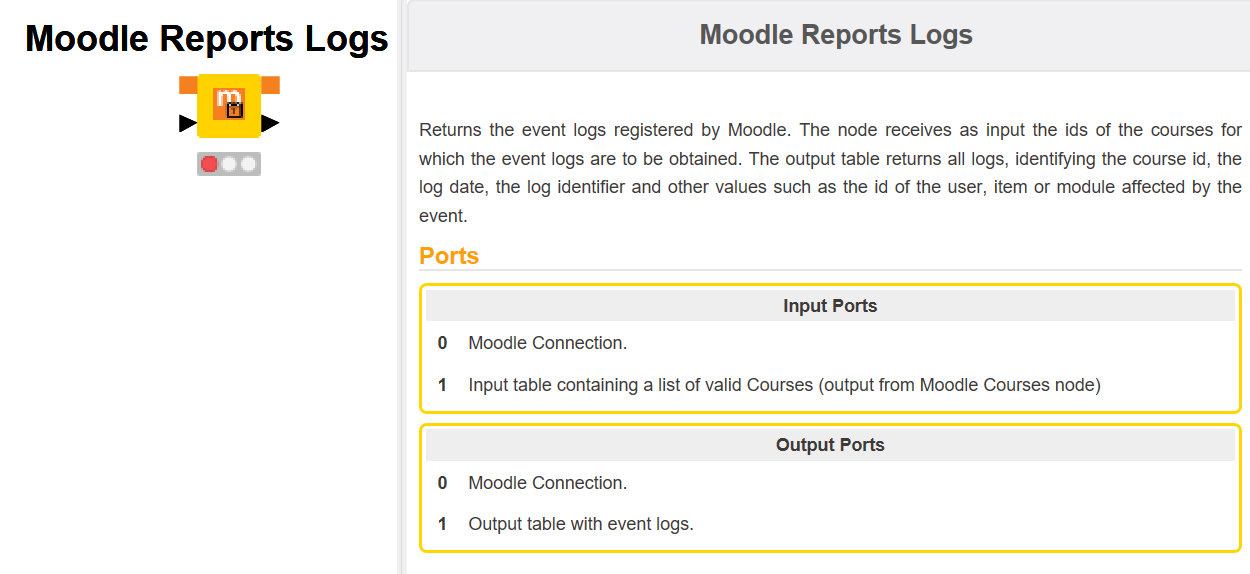
\includegraphics[width=1\textwidth]{img/nodes_moodle_reports_logs.png}
	\caption{Nodo \node{Moodle Reports Logs}. Descripción.}
	\label{fig:moodlereportslogs}
\end{figure}
\FloatBarrier

El nodo no tiene configuración específica. 
\

En la tabla~\ref{tab:moodle_reports_logs_desc} se muestra la estructura de los datos devueltos por cada evento del \english{log}: 

\begin{table}[!h]
	\begin{center}
		\begin{tabular}{p{0.3\textwidth}p{0.1\textwidth}p{0.6\textwidth}}
			\toprule
			\textbf{Columna} & \textbf{Tipo} & \textbf{Descripción}\\
			\otoprule
			\textbf{courseid} & integer & ID del curso \\
         \hline
			\textbf{time} & string & Fecha de registro del log en formato DD/MM/YYYY - HH:MM:SS +TimeZone. \\
         \hline
         \textbf{component} & string & Nombre del componente o módulo de Moodle que registra el evento \\
         \hline
         \textbf{eventName} & string & Nombre de sistema del evento \\
         \hline
         \textbf{origin} & string & Origen (WEB, CLI, APP, etc.) \\
         \hline
         \textbf{IPAddress} & string & Dirección IP del usuario \\
         \hline
         \textbf{course} & string & ID del curso extraído del mensaje de log \\
         \hline
         \textbf{user} & string & ID del usuario extraído del mensaje de log \\
         \hline
         \textbf{targetUser} & string & ID del usuario objetivo extraído del mensaje de log \\
         \hline
         \textbf{targetCourse} & string &  ID del curso objetivo extraído del mensaje de log \\
         \hline
         \textbf{module} & string &  ID del módulo extraído del mensaje de log \\
         \hline
         \textbf{section} & string &  ID de la sección extraído del mensaje de log \\
         \hline
         \textbf{item} & string &  ID del ítem extraído del mensaje de log \\
         \hline
         \textbf{description} & string & Mensaje completo guardado en el log \\
         \hline
         \textbf{descriptionMapped} & boolean &  Indica si el mensaje ha sido mapeado (1) o no (0)\\
         \hline
         \textbf{label} & string & Nombre del módulo (página, cuestionario, tarea, etc.) \\
         \bottomrule
		\end{tabular}
	\end{center}
	\caption{Tabla de salida del nodo \node{Moodle Reports Logs}.}
	\label{tab:moodle_reports_logs_desc}
\end{table}
\FloatBarrier

\begin{figure}[!h]
	\centering
	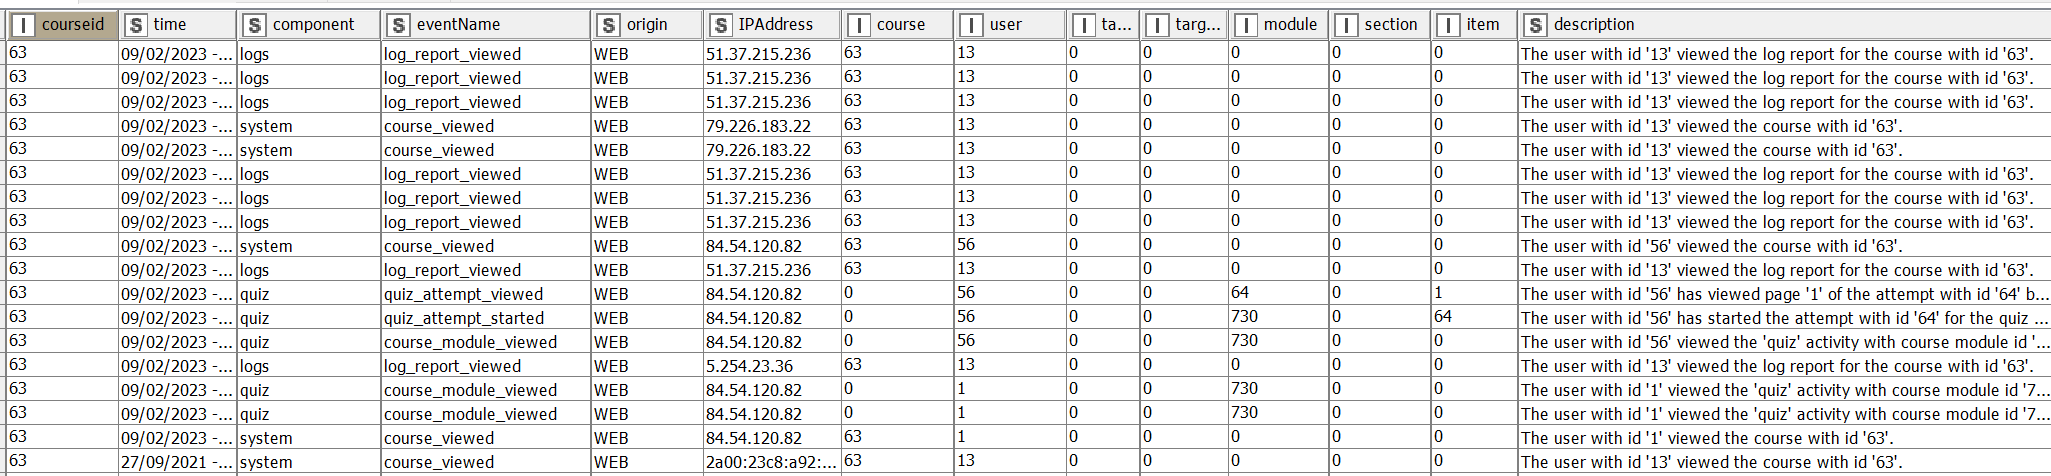
\includegraphics[width=1\textwidth]{img/nodes_moodle_reports_logs_output.png}
	\caption{Nodo \node{Moodle Reports Logs}. Salida.}
	\label{fig:moodlereportslogs_output}
\end{figure}
\FloatBarrier
\hphantom{ }




\newpage
\subsection{Diseño del nodo Moodle Reports Grades}

El nodo \node{Moodle Reports Grades} extrae información de calificaciones agrupadas por curso, estudiante y actividad (RF-5). Adicionalmente, devuelve una columna con la calificación final obtenida. 
\

El nodo tiene la siguiente \textbf{estructura}:

\begin{itemize}
	\item \textbf{Puertos de entrada}: 
    \begin{itemize}
		\item \textbf{0. Moodle Connection}. Conexión obtenida desde el nodo \node{Moodle Connector}. 
		\item \textbf{1. Input table}. Tabla de entrada con un listado de identificadores de cursos. 
   	\end{itemize}

	\item \textbf{Puertos de salida}: 
    \begin{itemize}
		\item \textbf{0. Moodle Connection}. Devuelve la conexión para facilitar su transferencia al siguiente nodo del flujo de trabajo. 
		\item \textbf{1. Output table}. Tabla de salida con la información de calificaciones. 
   	\end{itemize}

\end{itemize}

\begin{figure}[!h]
	\centering
	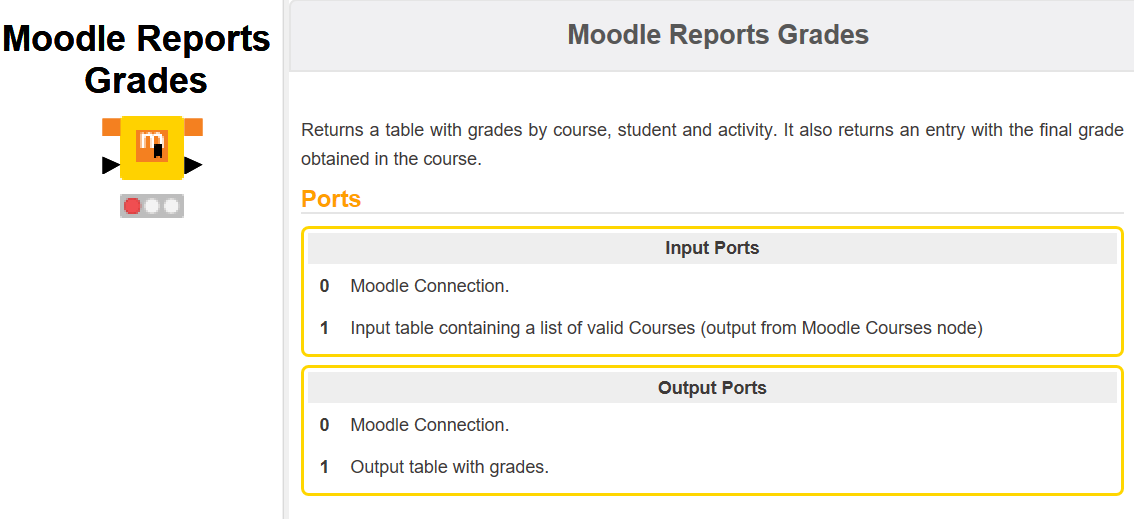
\includegraphics[width=1\textwidth]{img/nodes_moodle_reports_grades.png}
	\caption{Nodo \node{Moodle Reports Grades}. Descripción.}
	\label{fig:moodlereportsgrades}
\end{figure}
\FloatBarrier

El nodo no tiene configuración específica. 
\

En la tabla~\ref{tab:moodle_reports_grades_desc} se muestra la estructura de los datos devueltos por cada calificación, clasificada por curso/actividad/usuario: 

\begin{table}[!h]
	\begin{center}
		\begin{tabular}{p{0.25\textwidth}p{0.15\textwidth}p{0.6\textwidth}}
			\toprule
			\textbf{Columna} & \textbf{Tipo} & \textbf{Descripción}\\
			\otoprule
			\textbf{courseid} & integer & ID del curso en que está registrado el usuario \\
         \hline
			\textbf{userid} & integer & ID del usuario \\
         \hline
         \textbf{gradeid} & integer & ID de la calificación \\
         \hline
         \textbf{gradename} & string & Nombre de la actividad de calificación \\
         \hline
         \textbf{gradetype} & string & Tipo de calificación (mod, category, manual, course) \\
         \hline
         \textbf{grademodule} & string & Módulo de la actividad de calificación (assign, forum, quiz, etc.) \\
         \hline
         \textbf{grademin} & double & Valor mínimo de la calificación \\
         \hline
         \textbf{grademax} & double & Valor máximo de la calificación \\
         \hline
         \textbf{graderaw} & double & Calificación obtenida, sin formatear/procesar \\
         \hline
         \textbf{gradeformatted} & string & Calificación formateada \\
         \hline
         \textbf{gradecategoryid} & integer & ID de categoría de calificación \\
         \bottomrule
		\end{tabular}
	\end{center}
	\caption{Tabla de salida del nodo \node{Moodle Reports Grades}.}
	\label{tab:moodle_reports_grades_desc}
\end{table}
\FloatBarrier

\begin{figure}[!h]
	\centering
	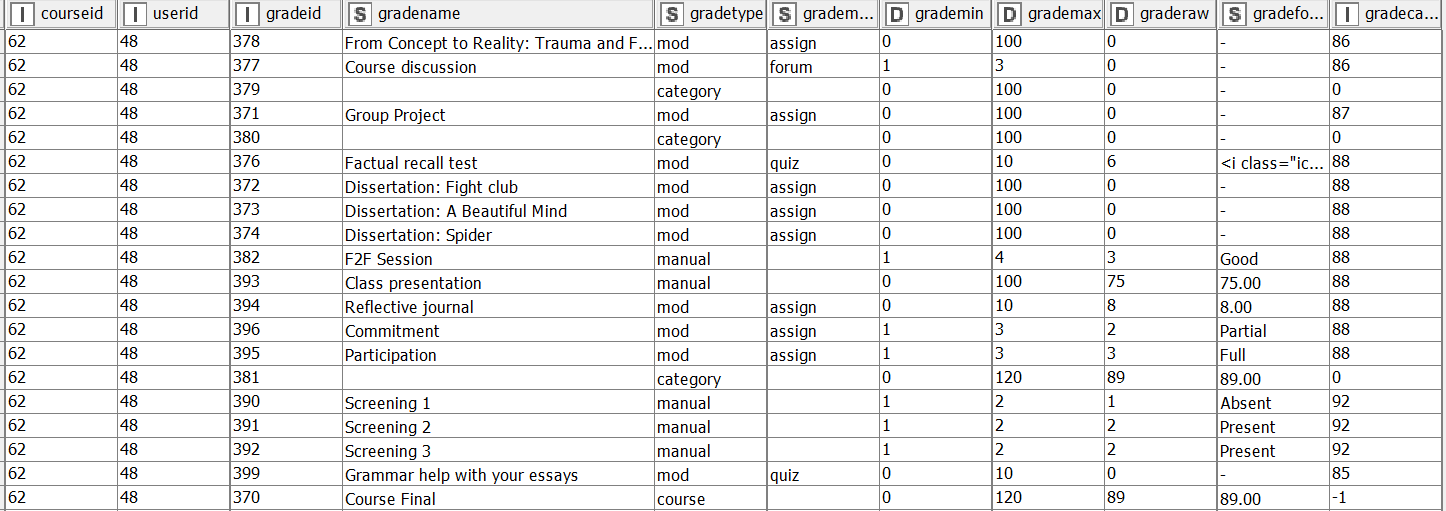
\includegraphics[width=1\textwidth]{img/nodes_moodle_reports_grades_output.png}
	\caption{Nodo \node{Moodle Reports Grades}. Salida.}
	\label{fig:moodlereportsgrades_output}
\end{figure}
\FloatBarrier
\hphantom{ }


\newpage
\subsection{Diseño del nodo Moodle Reports Quizzes}

El nodo \node{Moodle Reports Quizzes} extrae información sobre los intentos realizados por los estudiantes en los cuestionarios (RF-6). 
\

El nodo tiene la siguiente \textbf{estructura}:

\begin{itemize}
	\item \textbf{Puertos de entrada}: 
    \begin{itemize}
		\item \textbf{0. Moodle Connection}. Conexión obtenida desde el nodo \node{Moodle Connector}. 
		\item \textbf{1. Input table}. Tabla de entrada con un listado de identificadores de cursos. 
   	\end{itemize}

	\item \textbf{Puertos de salida}: 
    \begin{itemize}
		\item \textbf{0. Moodle Connection}. Devuelve la conexión para facilitar su transferencia al siguiente nodo del flujo de trabajo. 
		\item \textbf{1. Output table}. Tabla de salida con la información sobre los intentos realizados en cuestionarios. 
   	\end{itemize}

\end{itemize}


\begin{figure}[!h]
	\centering
	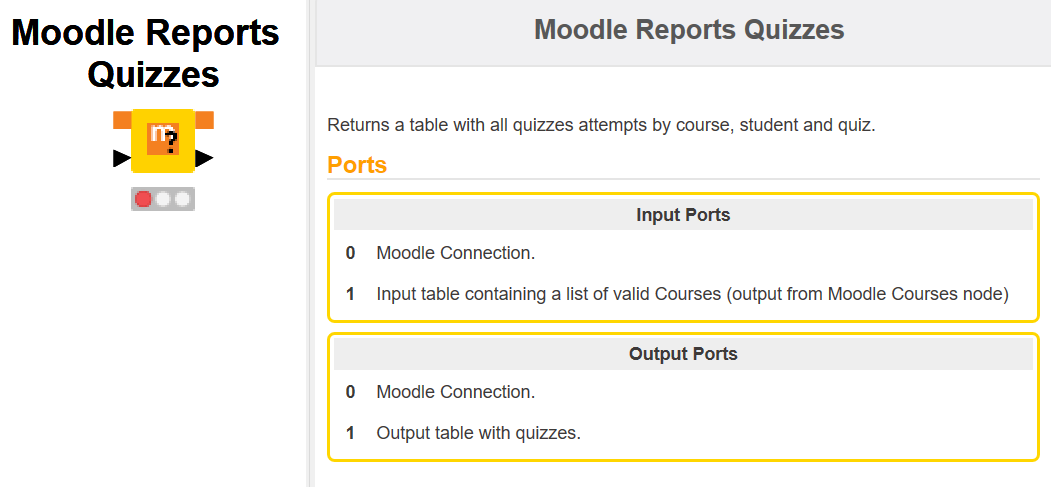
\includegraphics[width=1\textwidth]{img/nodes_moodle_reports_quizzes.png}
	\caption{Nodo \node{Moodle Reports Quizzes}. Descripción.}
	\label{fig:moodlereportsquizzes}
\end{figure}
\FloatBarrier


El nodo no tiene configuración específica. 
\

En la tabla~\ref{tab:moodle_reports_quizzes_desc} se muestra la estructura de los datos devueltos por cada intento de realización de cuestionario: 

\begin{table}[!h]
	\begin{center}
		\begin{tabular}{p{0.25\textwidth}p{0.15\textwidth}p{0.6\textwidth}}
			\toprule
			\textbf{Columna} & \textbf{Tipo} & \textbf{Descripción}\\
			\otoprule
			\textbf{courseid} & integer & ID del curso en que está registrado el usuario \\
         \hline
			\textbf{userid} & integer & ID del usuario \\
         \hline
         \textbf{coursemoduleid} & integer & ID del módulo \\
         \hline
		 \textbf{quizid} & integer & ID del cuestionario \\
         \hline
         \textbf{quizname} & string & Nombre del cuestionario \\
         \hline
		 \textbf{attemptid} & integer & ID del intento de resolución del cuestionario \\
         \hline
		 \textbf{attemptnumber} & integer & Número del intento de resolución del cuestionario \\
         \hline
		 \textbf{attemptduration} & integer & Duración del intento en segundos \\
         \hline
         \textbf{attemptgrade} & double & Calificación obtenida en este intento \\
         \bottomrule
		\end{tabular}
	\end{center}
	\caption{Tabla de salida del nodo \node{Moodle Reports Quizzes}.}
	\label{tab:moodle_reports_quizzes_desc}
\end{table}
\FloatBarrier


\begin{figure}[!h]
	\centering
	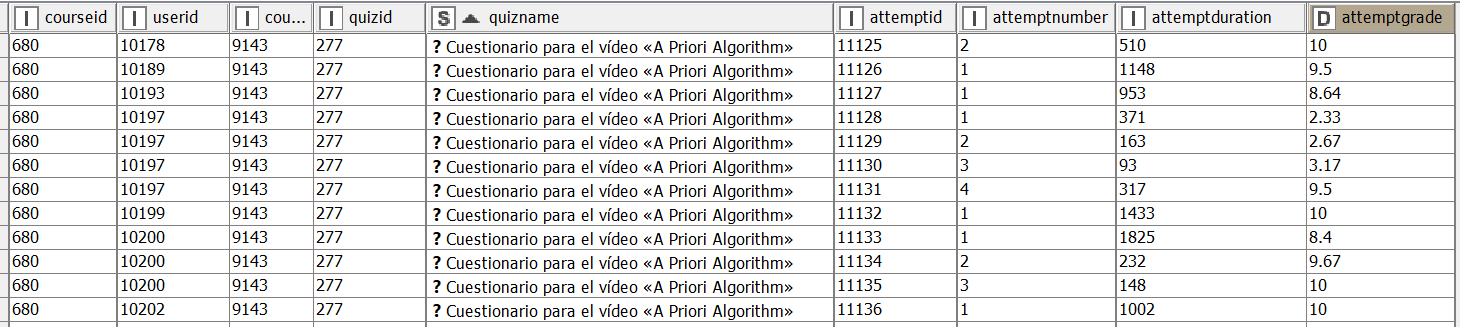
\includegraphics[width=1\textwidth]{img/nodes_moodle_reports_quizzes_output.png}
	\caption{Nodo \node{Moodle Reports Quizzes}. Salida.}
	\label{fig:moodlereportsquizzes_output}
\end{figure}
\FloatBarrier
\hphantom{ }


